% 2D Image with indices
% Author: Peter Steinbach
\documentclass[tikz]{standalone}
%\documentclass[dvisvgm]{standalone}
%\def\pgfsysdriver{pgfsys-tex4ht.def}
\usepackage{units}
\usepackage{tikz}
\usetikzlibrary{calc,math,trees,positioning,arrows.meta,chains,shapes.geometric,shapes.arrows,%
    decorations.pathreplacing,decorations.pathmorphing,shapes,%
    matrix,shapes.symbols,fit,backgrounds}

 \pgfdeclarelayer{back}
 \pgfsetlayers{background,back,main}


\makeatletter
\makeatother

\begin{document}
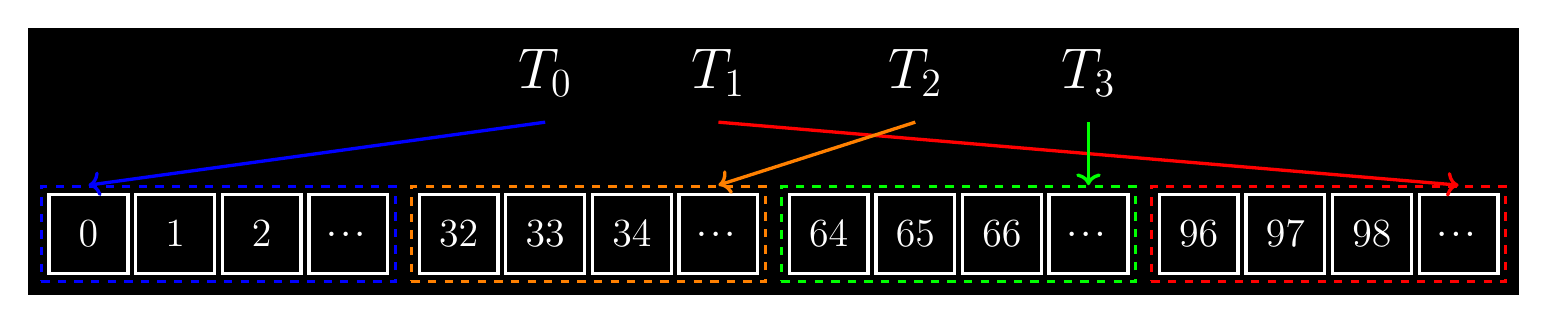
\begin{tikzpicture}[
  show background rectangle, 
  background rectangle/.style={fill=black},
  color=white,
  help lines/.style={color=lightgray,line width=.2pt},
  ]

  \node (line_0) [rectangle,dashed,draw=white,very thick,minimum width=4.5cm,minimum height=1.2cm,anchor=west,draw=blue] at($(0,0)+(0,0)$) {};
  \node (line_1) [rectangle,dashed,draw=white,very thick,minimum width=4.5cm,minimum height=1.2cm,anchor=west,draw=orange] at($(0,0)+(4.7*1,0)$) {};
  \node (line_2) [rectangle,dashed,draw=white,very thick,minimum width=4.5cm,minimum height=1.2cm,anchor=west,draw=green] at($(0,0)+(4.7*2,0)$) {};
  \node (line_3) [rectangle,dashed,draw=white,very thick,minimum width=4.5cm,minimum height=1.2cm,anchor=west,draw=red] at($(0,0)+(4.7*3,0)$) {};


  \foreach \c in {0,...,3}
   {
     % %cache line
     % \tikzmath{
     %   integer \id;
     %   \id = 3*\c;
     % }

     \foreach \n in {0,...,2}
     {
       \tikzmath{
         integer \id, \m;
         \id = (4*\c)+\n;
         \m = (32*\c)+\n;
       }
         
       \node (mem_\id) [rectangle,draw=white,very thick,minimum width=1.cm,minimum height=1.cm,anchor=west,font=\Large] at($(line_\c.west)+(.1,0) + (1.1*\n,0)$) {$\m$};
     
     }
     
     \tikzmath{
         integer \id;
         \id = (4*\c)+3;
       }
       \node (mem_\id) [rectangle,draw=white,very thick,minimum width=1.cm,minimum height=1.cm,anchor=west] at($(line_\c.west)+(3.4,0)$) {\bfseries{}\dots};
   }
  
   \node (thread_0) [draw=none,font=\huge,above] at($(mem_5.north) + (0,1.1)$) {$T_{0}$};
   \draw[->,very thick,draw=blue] ($(thread_0.south) + (0,-.2)$) -- ($(mem_0.north) + (0,.1)$);
   
   \node (thread_1) [draw=none,font=\huge,above] at($(mem_7.north) + (0,1.1)$) {$T_{1}$};
   \draw[->,very thick,draw=red] ($(thread_1.south) + (0,-.2)$) -- ($(mem_15.north) + (0,.1)$);

   \node (thread_2) [draw=none,font=\huge,above] at($(mem_9.north) + (0,1.1)$) {$T_{2}$};
   \draw[->,very thick,draw=orange] ($(thread_2.south) + (0,-.2)$) -- ($(mem_7.north) + (0,.1)$);
   
   \node (thread_3) [draw=none,font=\huge,above] at($(mem_11.north) + (0,1.1)$) {$T_{3}$};
   \draw[->,very thick,draw=green] ($(thread_3.south) + (0,-.2)$) -- ($(mem_11.north) + (0,.1)$);
   
\end{tikzpicture}
\end{document}
